\let\textcircled=\pgftextcircled
\chapter{The LHC and the CMS experiment}
\label{chap:detector}

\initial{T}his is the detector chapter.

%=======
\begin{easylist}[itemize]
\ListProperties(Style*=-- , FinalMark={)}, Margin=0.5cm)
& Explain \acrshort{cern} and the \acrshort{lhc} in more detail.
& Give an overview of the \acrshort{cms} experiment and detector (including all subsystems, object identification, algorithms for event/object reconstruction like Particle Flow and \gls{antikt}, and algorithms for tagging objects like \glspl{bjet}).
& Either as a subsection in this chapter or in a separate chapter, discuss the Level-1 Trigger in depth. Emphasise the jet and energy sum triggers as I've worked on them, and Calorimeter Layer-2 for the same reason.
\end{easylist}

\section{The Large Hadron Collider}

Deep underground beneath the Franco-Swiss border lies the \acrfull{lhc}, a synchrotron particle accelerator 27~km in circumference. Predominantly a proton collider, lead and xenon ions have also been injected for novel and unique studies. Four principle experiments are situated at their own interaction points where the two beams of particles are brought into contact: \acrfull{cms}, a general purpose detector with interests in precision measurements, searches for new physics, and many other avenues; \acrshort{atlas} (\acrlong{atlas}), another general purpose detector with similar aims to \acrshort{cms}; LHCb, designed to study the decay of \PB hadrons; and \acrshort{alice} (\acrlong{alice}), primarily studying heavy ion collisions and the quark-gluon plasma.

% Describe the structure of the LHC - beam pipe, magnets, cooling, feeding in to LHC from PS/SPS, etc., beam structure (train of bunches, 11k revolutions around ring per second), bunch interaction/collision (40 MHz bunch collision frequency, crossing angle) 

The \acrshort{lhc} began operating in 2010 at a centre of mass energy of $\sqrt{s} = \text{7}\TeV$ (\acrlong{tev}s), 3.5\TeV per beam. A modest increase to 8\TeV was achieved by the end of Run-1 in 2013. After upgrades were performed, the LHC resumed operation in 2015, further pushing the frontiers of high energy physics with a centre of mass energy of \comruntwo. While valuable data was taken, it was not until 2016 when Run-2 of the \acrshort{lhc} began. This period ended in 2018 with 162.85\fbinv of $\Pp\Pp$ collisions delivered, 150.26\fbinv of which were recorded by \acrshort{cms}.


\section{The CMS experiment}

\begin{figure}[htbp]
\centering
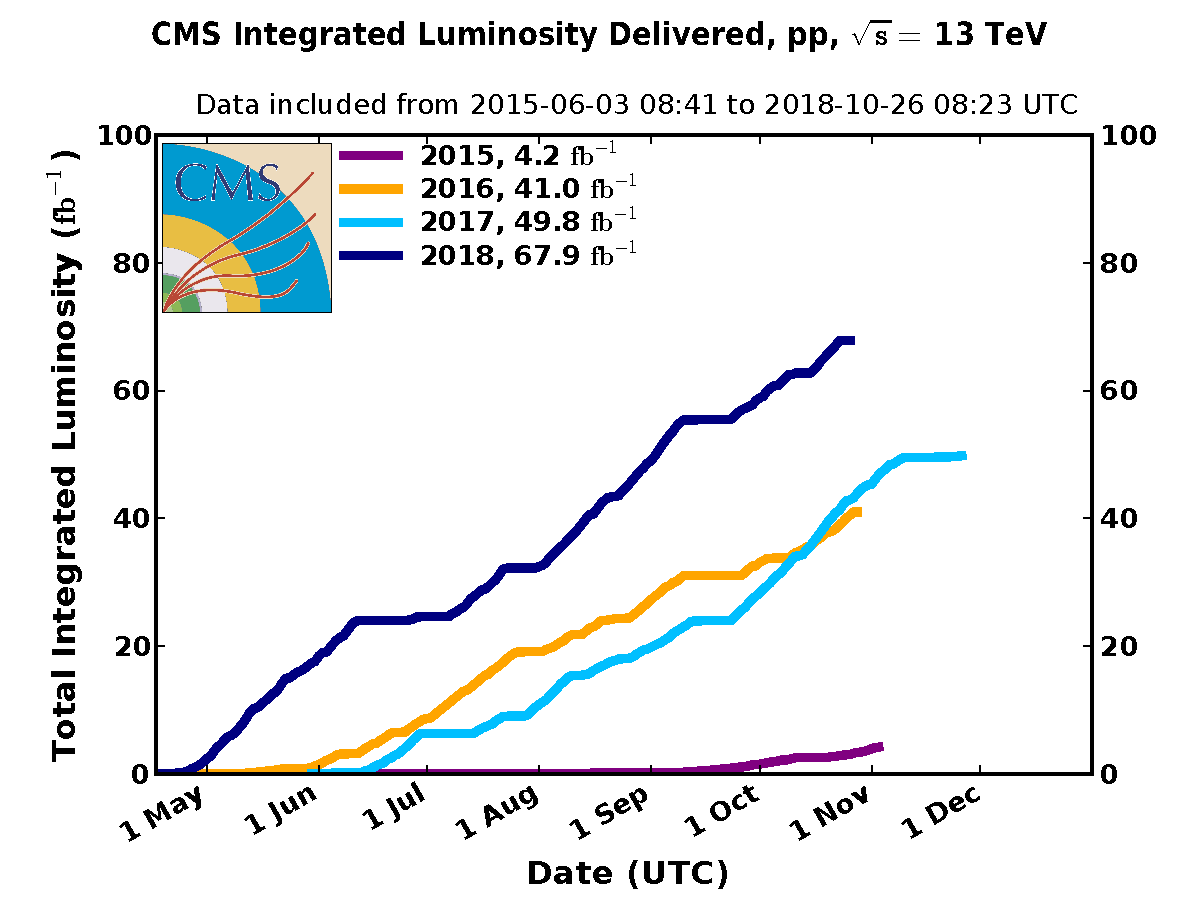
\includegraphics[width=0.75\textwidth]{figures/int_lumi_cumulative_pp_2_run2.pdf}
\caption{The integrated luminosity of $\Pp\Pp$ collision data collected by CMS during 2015 and Run-2 of the LHC \cite{cmslumitwikipage}.}
\end{figure}

\begin{figure}[htbp]
\centering
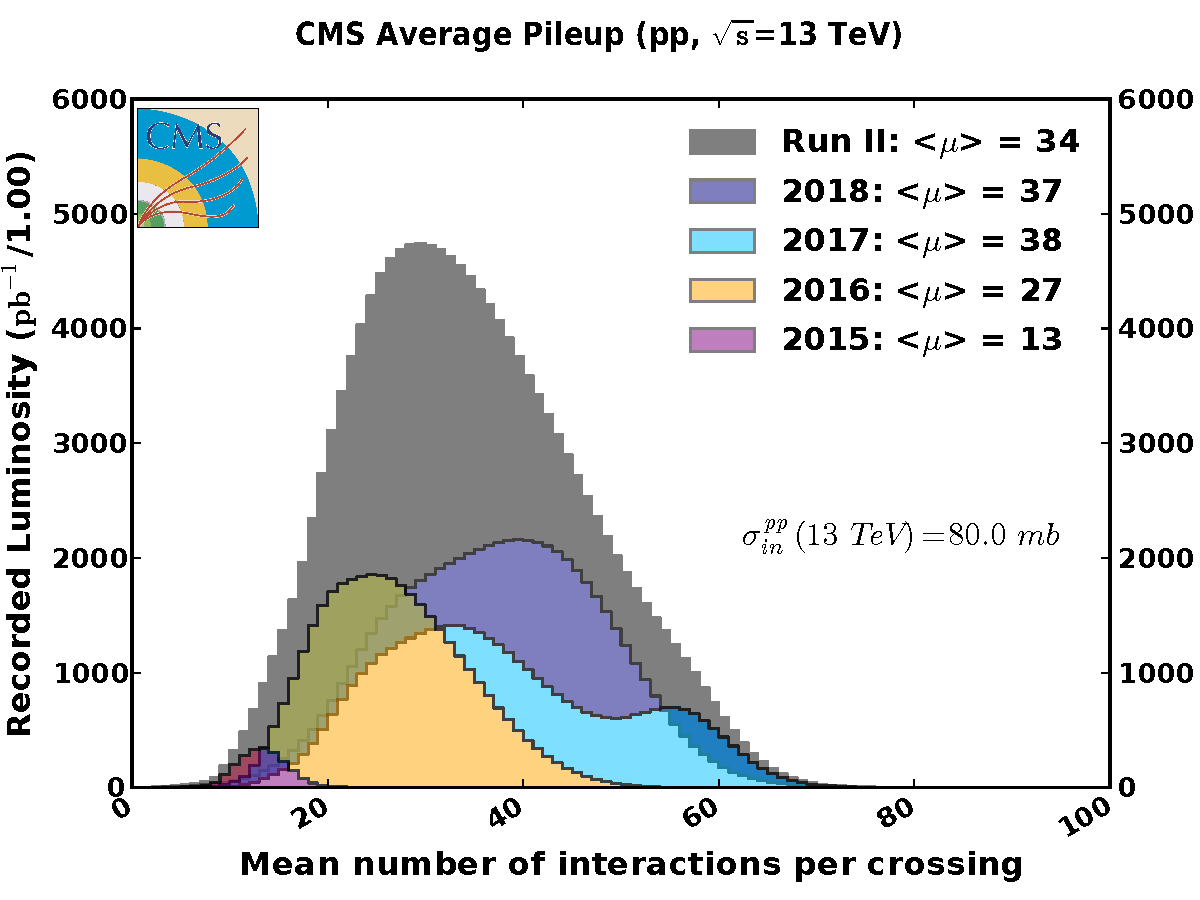
\includegraphics[width=0.75\textwidth]{figures/pileup_allYears_run2.pdf}
\caption{The average number of pileup interactions at CMS during 2015 and Run-2 of the LHC \cite{cmslumitwikipage}.}
\end{figure}

\subsection{Jet energy corrections in the Level-1 Trigger}
